\documentclass{article}
\usepackage[utf8]{inputenc}
\usepackage[brazil]{babel}
\usepackage{graphicx}
\graphicspath{ {imgs/} }
\usepackage{mathtools}
\usepackage[colorinlistoftodos,prependcaption,textsize=tiny]{todonotes}
\usepackage[hypcap=true]{caption}
\usepackage[colorlinks, linkcolor=blue, urlcolor=blue, citecolor=blue]{hyperref}
\usepackage[a4paper, left=20mm, right=20mm, top=20mm, bottom=20mm]{geometry}

\title{\textbf{INE5421 - Linguagens Formais e Compiladores \\
        \large Trabalho T1 - Manipulador de LR representadas por AF e ER}}
\author{
    Caique Rodrigues Marques \\
    {\texttt{c.r.marques@grad.ufsc.br}}
    \and
    Fernando Jorge Mota \\
    {\texttt{contato@fjorgemota.com}}
    \vspace{-5mm}
}
\date{}

\begin{document}

\maketitle

\section{Introdução}
    O software possibilita a verificação e a execução de operações relacionadas
    a autômatos finitos e expressões regulares, através de simples operações é
    possível verificar a equivalência de dois autômatos finitos, o autômato
    finito equivalente a uma dada expressão regular, a diferença entre dois
    autômatos finitos e entre outras operações que serão detalhadas no decorrer
    deste relatório.

\section{Uso do Programa}
\label{sec:uso}
    Ao iniciar o programa, ilustrado na figura \ref{fig:start_point}, uma
    janela conterá uma aba com a mensagem de boas-vindas com um pequeno resumo
    de quais passos básicos seguir para a execução do software. Na tela inicial
    do software também contém três menus na parte superior da janela:
    \texttt{File}, \texttt{Operations} e \texttt{Tab}, a seguir será detalhado
    mais sobre os três menus.

    \begin{figure}[htp]
        \centering
        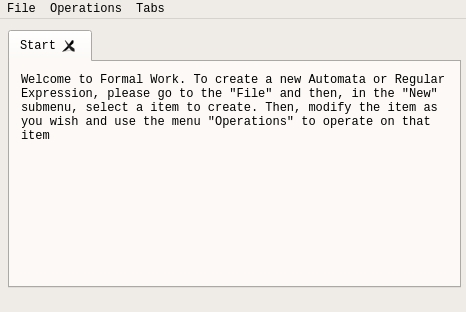
\includegraphics[width=.7\linewidth]{print_program.jpg}
        \caption{Tela inicial do software}
        \label{fig:start_point}
    \end{figure}

    \begin{itemize}
        \item \texttt{\textbf{File}}: este menu contém duas opções:
            \texttt{New} e \texttt{Exit}, a primeira opção permite a criação de
            um novo conjunto regular, ao selecionar a opção, um novo submenu
            aparece possibilitando a criação de um autômato finito
            (\texttt{Finite Automata}) ou de uma expressão regular (Regular
            Expression). Clicando em qualquer um, uma nova janela aparecerá
            fornecendo um campo digitável para a escrita do nome do conjunto
            regular a ser criado; a segunda opção é para sair do programa.

        \item \texttt{\textbf{Operations}}: Permite realizar as operações entre
            os conjuntos regulares, tais operações são detalhadas na seção
            relacionada à implementação (\ref{sec:imp}). Este menu contém um
            submenu divido por uma linha, onde a parte superior corresponde às
            operações envolvendo autômatos finitos e a outra envolvendo
            operações com expressões regulares. Vale citar que dada uma
            expressão regular, ela será transformada em um autômato finito via
            algoritmo de Simone (\ref{subsec:desimone}) e, assim, conseguirá
            realizar a todas as operações relacionadas a autômatos finitos.
 
        \item \texttt{\textbf{Tab}}: Menu relacionado a aba em que se está
            trabalhando, contendo duas opções: \texttt{Change Name} e
            \texttt{Duplicate}. A primeira opção permite a mudança de nome da
            aba, obviamente, tal mudança só será aceita se for um nome único,
            que não tenha sido utilizado em outra aba; a segunda opção permite
            a duplicação de conteúdo, ou seja, o conteúdo da aba é copiado para
            uma nova, com um outro nome que pode ser escolhido pelo usuário.
    \end{itemize}
 
\section{Operações}
    \subsection{Operações com autômatos finitos}
        O foco do software está na manipulação de expressões regulares e
        autômatos finitos, portanto, como já descrito na seção anterior
        (\ref{sec:uso}) o menu \texttt{Operations} contém as operações para
        manipulação dos conjuntos regulares. As operações possíveis para
        autômatos finitos são:

        \begin{enumerate}
            \item \texttt{Union} (União)
            \item \texttt{Intersection} (Interseção)
            \item \texttt{Difference} (Diferença)
            \item *\texttt{Complement} (Complemento)
            \item \texttt{Containment} (Contenção)
            \item \texttt{Equivalence} (Equivalência)
            \item *\texttt{Check if accept} (Checar se aceita)
            \item *\texttt{Determinize} (Determinização)
            \item *\texttt{Minimize} (Minimização) 
        \end{enumerate}

        As operações com * são operações que funcionam com apenas um autômato
        como entrada, ou seja, não requisitam outro autômato ou expressão
        regular e simplesmente geram a entrada solicitada. Note que todas as
        operações exigem autômatos finitos ou expressões regulares válidas,
        caso contrário, o software irá destacar em amarelo o problema com o
        autômato e, ao passar o cursor na região em destaque, na parte inferior
        da janela irá detalhar qual o problema relatado. A figura
        \ref{fig:2data} ilustra dois avisos diferentes notados pelo software.

        \begin{figure}[!h]
            \centering
            \begin{minipage}[b]{.4\textwidth}
                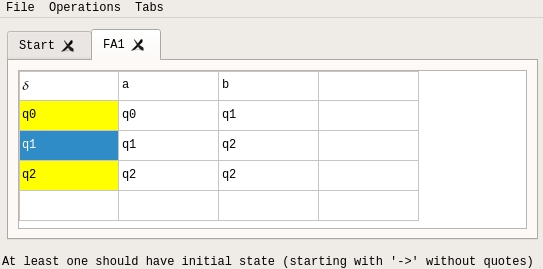
\includegraphics[width=\textwidth]{print_warn1.jpg}
            \end{minipage}
            \begin{minipage}[b]{.4\textwidth}
                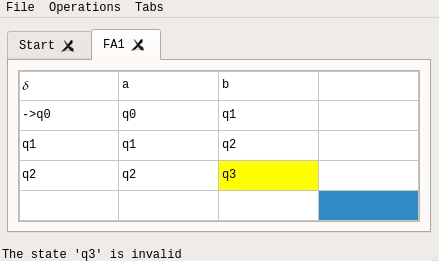
\includegraphics[width=\textwidth]{print_warn2.jpg}
            \end{minipage}
            \caption{Dois exemplos de avisos apontados pelo software. À
            esquerda está o aviso da falta de um estado inicial na criação de
            um autômato, à direita descreve sobre a inexistência de um estado.}
            \label{fig:2data}
        \end{figure}

        Com exceção da operação de número 7 da lista, todas as operações
        realizadas explicitam os passos usados para a geração da saída
        especificada, na figura \ref{fig:intersec} ilustra o resultado de uma
        interseção entre a expressão regular $(a|b)^{*}b^{+}(c)^{?}$ e o
        autômato finito de teste gerado ao iniciar o software. Cada passo
        intermediário apresentado pelo software vem acompanhado de um botão
        \texttt{Move to tab}, que permite que o autômato em questão seja
        copiado para um nova aba e, assim, seja trabalhado em particular.

        \begin{figure}[htp]
            \centering
            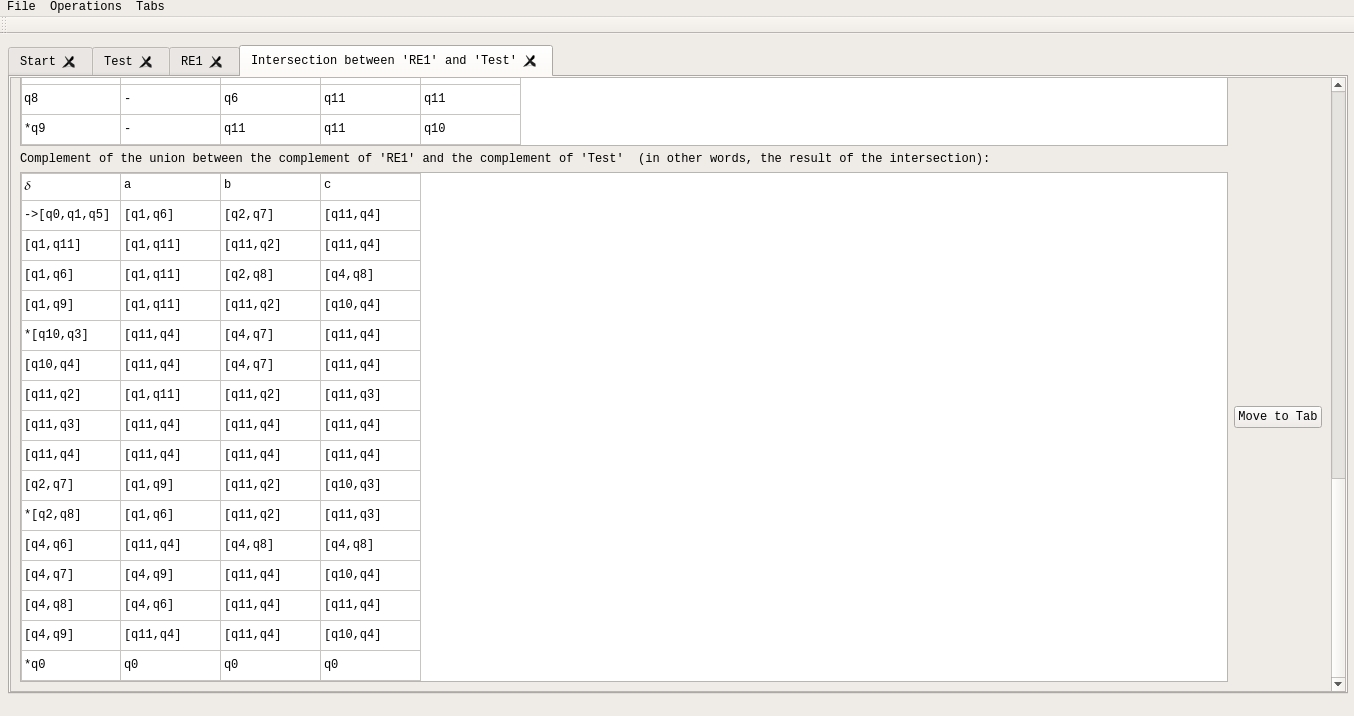
\includegraphics[width=.7\linewidth]{print_intersection.jpg}
            \caption{Resultado da interseção de uma expressão regular com um
            autômato finito}
            \label{fig:intersec}
        \end{figure}

    \subsection{Operações com expressões regulares}
        A única operação possível que envolve diretamente expressões regulares
        está na transformação delas em um autômato finito. Assim, tendo um
        autômato equivalente à expressão regular, é possível realizar as
        operações listadas na seção anterior.

\section{Implementação}
\label{sec:imp}
    \subsection{Autômatos Finitos}
        Todas as operações relacionadas aos autômatos finitos estão
        explicitadas na classe \texttt{FiniteAutomata}. A seguir, um
        detalhamento das operações relacionadas aos autômatos finitos.

        \subsubsection{Propriedades básicas de autômatos finitos}
            O conjunto de autômatos finitos regulares são fechados a quatro
            operações: união, complemento, concatenação e interseção. Tais
            operações básicas possibilitam a realização de outras operações
            como a diferença, equivalência e contenção. A seguir é apresentado
            como o software consegue realizar tais operações partindo das
            propriedades básicas.
            \begin{itemize}
                \item \textbf{Diferença}: A diferença de dois autômatos finitos
                    regulares T1 e T2 é equivalente a $T1 \cap \overline{T2}$
                    que é equivalente a $\overline{\overline{T1} \cup T2}$
                    (prova por teorema de De Morgan);

                \item \textbf{Interseção}: A interseção de dois autômatos
                    finitos regulares T1 e T2 é equivalente a
                    $\overline{\overline{T1} \cup \overline{T2}}$ (prova por
                    teorema de De Morgan);

                \item \textbf{Contenção}: Dados dois autômatos finitos
                    quaisquer T1 e T2, $T1 \subseteq T2 \leftrightarrow T1 \cap
                    \overline{T2} = \varphi$;

                \item \textbf{Equivalência}: Dados dois autômatos finitos T1 e
                    T2 quaisquer, $T1 = T2 \leftrightarrow T1 \subseteq T2 \and
                    T2 \subseteq T1$.3
            \end{itemize}

        \subsubsection{Determinização de um autômato finito}
            Um autômato é dito não determinístico se ele possui pelo menos um
            estado cujas transições levam a dois estados diferentes por um
            mesmo símbolo do alfabeto. A determinização de um autômato finito
            não determinístico acontece definindo cada a transição de cada
            estado e, quando um símbolo leva a dois estados diferentes, estes
            são unidos, formando um só - tais etapas são repetidas ate que
            todas as transições do autômato finito sejam determinísticas.

        \subsubsection{Minimização de um autômato finito}
            Um autômato finito é dito mínimo se ele não possui estados mortos,
            não possui estados inalcançáveis e não possui estados equivalentes,
            assim, para a minimização de um autômato qualquer as três condições
            devem ser seguidas.

            A remoção de estados mortos é feita a partir da verificação de cada
            estado, se um estado não possui transições de saída e não é estado
            final, então, ele é considerado morto e é removido, retornando um
            novo autômato finito sem estados mortos. Para remoção de estados
            inalcançáveis é feita uma varredura no autômato, partindo do estado
            inicial seguindo todas as transições possíveis, o novo autômato é
            retornado contendo apenas os estados que foram alcançados por essa
            varredura.

            Para o último passo para a minimização de um autômato finito é a
            remoção dos estados equivalentes. Como primeiro passo, os estados
            são divididos em duas classes (grupos) de equivalência: de estados
            finais e de estados não finais, logo em seguida, cada estado tem
            suas transições verificadas, se um ou mais estados do mesmo tipo
            ```apontam" para o mesmo grupo, então eles são agrupados numa mesma
            classe de equivalência. Após, novamente cada estado é avaliado e se
            a condição novamente for verdadeira em relação ao então número de
            classes de equivalência, novas são formadas, assim segue
            sucessivamente até que todos os estados equivalentes estejam
            devidamente agrupados. Esses novos grupos formam um único estado e,
            assim, é retornado o autômato finito sem estados equivalentes.

    \subsection{Expressão Regular}
        Todas as operações relacionadas às expressões regulares estão
        explicitadas na classe \texttt{RegularExpression}. A seguir, as
        operações relacionadas às expressões regulares.

        \subsubsection{Árvore associada}
            Dada uma expressão regular, sempre é possível associá-lo a uma
            árvore binária, esta é formada a partir das operações de menor para
            maior prioridade. A árvore associada à expressão regular acaba
            sendo útil para a obtenção do autômato finito associado à mesma
            expressão regular, usando-se o algoritmo baseado no método de
            Simone que será detalhado na subseção posterior.

            Para a obtenção da árvore associada à expressão regular, primeiro a
            expressão em si é normalizada, ou seja, todas as operações se
            tornam explícitas, por exemplo, a expressão regular
            $(ab)^{*}(ba)^{+}$ possui forma normalizada como
            $(a.b)^{*}.(b.a)^{+}$. A seguir, a expressão regular é examinada e
            é coletada a operação de menor prioridade, da esquerda para a
            direita e fora de parênteses, como nó raiz da árvore, disto, também
            é definido os nós filhos desse nó raiz - no exemplo citado, ``$.$"
            será a raiz e as subexpressões ``$(a.b)^{*}$" e ``$(b.a)^{+}$"
            serão os nós filhos à esquerda e à direita, respectivamente, de
            ``$.$".

            O algoritmo de obtenção da árvore associada é recursivo, assim, as
            subexpressões serão analisadas da mesma forma descrita antes. O
            algoritmo para quando não há mais subexpressões para analisar.

        \subsubsection{Método de Simone}
        \label{subsec:desimone}
            O método de Simone possibilita a transformação de uma expressão
            regular qualquer a um autômato finito associado, tal autômato
            resultante não necessariamente é mínimo. A execução deste algoritmo
            começa com a obtenção de uma árvore de Simone associada à expressão
            regular, os resultados gerados pelo algoritmo serão provindos por
            informações obtidas nesta árvore; em seguida, a partir da árvore, é
            coletada as composições que são formadas partindo de cada nó folha,
            estas composições serão úteis posteriormente; o primeiro
            percorrimento da árvore é feito, assim, é gerado o primeiro estado
            (normalmente nomeado como "\texttt{q0}") e a primeira composição de
            nó folhas deste estado inicial, disto é possível inferir por quais
            símbolos \texttt{q0} terá transições.

            Para os estados posteriores, não é necessário nenhum percorrimento
            à arvore de Simone, pois, com as composições alcançadas por nós
            folhas coletadas no começo do algoritmo, é necessário apenas
            detalhar a composição do estado partindo das composições
            alcançáveis já conhecidas. Assim, durante esses passos, é criado o
            estado em questão e suas transições já são definidas a partir de
            suas composições. Vale citar que o algoritmo já trata de casos
            onde, se a composição de dois estados forem exatamente iguais, um é
            automaticamente descartado evitando a inclusão de estados
            equivalentes (quaisquer referências a equivalentes, sempre serão
            associadas ao primeiro estado que teve tal composição). Após todo o
            processamento da composição dos estados, resultará no autômato
            finito equivalente, que será o retorno deste algoritmo.

            Uma observação em questão de implementação, o algoritmo também
            trata casos onde o método pode resultar em \textit{loops}
            infinitos, como por exemplo as expressões regulares $((a^{*})^{*})$
            e $(1|0)^{?}((10)^{*}(01)^{*})^{*}(1|0)^{?}$. Essa verificação é
            feita usando uma fila de ações já realizadas em um nó (rotinas de
            subida ou descida), portanto, uma ação não é repetida duas vezes
            por um mesmo nó.

    \section{Testes realizados}
        Toda a validação das estruturas que compõem o programa foram feitas
        usando testes unitários, para isto foi utilizado o framework
        gtest\footnote{\href{https://github.com/google/googletest}{Google Test}
        - Framework para testes de códigos em C++}. No total, foram realizados
        49 testes unitários para autômatos finitos e 22 testes unitários para
        expressões regulares, muitos desenvolvidos de maneira iterativa
        conforme os métodos foram sendo criados e problemas foram encontrados.
        Além disso, um serviço denominado Travis
        CI\footnote{\href{https://travis-ci.com}{Travis CI} - Serviço de
        integração contínua} testou cada commit realizado no projeto,
        compilando e realizando os testes em plataformas como o Linux e o
        macOS, de forma a garantir que problemas fossem encontrados rapidamente
        no código.
\end{document}
